\section{Method}
\label{SECII}\label{sec:method}
\subsection{The standard approach: matched filtering}

Searches for gravitational waves from compact binary coalescences typically
employ matched filter banks \cite{findchirppaper}.  Potential inspiral signals
are continuously parameterized by time, amplitude, phase, and a set of
intrinsic source parameters $\theta$, which in this paper we shall take to
consist of the two component masses of a binary, $\theta = (m_1, m_2)$.  Let
$h_+(\theta)$ and $h_\times(\theta)$ be, respectively, the `$+$' and `$\times$'
polarization gravitational wave signals that would arise from a fiducial
face-on binary at some distance.  Because, for inspiral signals, $h_+$ and
$h_\times$ are nearly in quadrature, they are generally combined into a single
complex-valued template $h = h_+ + i h_\times$.

The detection procedure for just one set of intrinsic source parameters
$\theta$ starts by {\em whitening} the measurement data stream $x$.  This
involves finding a linear filter that renders the detector's noise \textsc{iid}
and Gaussian.  This filter is applied to the measurement, yielding the whitened
data stream $x^\mathrm W$.  The same linear filter is applied to the template
$h(\theta)$, yielding the whitened template $h^\mathrm W (\theta)$.  The
matched filter is the normalized cross-correlation of $h^\mathrm W$ and
$x^\mathrm W$, \editorial{After introducing the $\star$ notation for cross
correlation, must we define it for continuous and discrete time?}
%
$$
%
\rho(\theta) = \frac{h^\mathrm W (\theta) \star x^\mathrm W}{|h^\mathrm W
(\theta)|}.
%
$$
%
This is called the signal to noise ratio, or \textsc{snr}.  The detection
statistic is the modulus of this, $|\rho(\theta)|$, which has a $\chi^2$
distribution with 2 degrees of freedom in the absence of signal.

To construct a filter bank, matched filters are realized for discrete signal
parameters $\theta_1,\, \theta_2,\, \cdots$, $\theta_N$, such that any possible
signal will have a maximum cross-correlation of at least 0.97 with at least one
template.  \editorial{Citation needed for template placement procedure?}  Such
a template bank is said to have a 97\% {\em minimum match}.  This technique is
designed so that an inspiral signal can be detected without any prior knowledge
of its intrinsic parameters: at most 3\% of the \textsc{snr} is lost by a
signal's parameters not exactly coinciding with a template's.  A trigger is
reported for the template parameters $\theta_i$ and time $t$ for which $|\rho|$
is a maximum over some moving interval in $\theta$ and $t$.

\subsubsection{Latency and overhead}

The matched filter bank can be implemented with finite impulse response
(\textsc{fir}) filters.  \textsc{fir} filters are perfectly suited for realtime
detection, because they do not introduce any latency at all.  However,
\textsc{fir} filters are very expensive: for $N$ templates of $M$ samples each,
a \textsc{fir} matched filter bank costs $\mathcal O(M N)$ operations per
sample.

Much more commonly, the matched filter bank is implemented using \textsc{fft}
convolutions, costing only $\mathcal O(M \lg N)$ \editorial{$\lg$ is $\log_2$.
Explain nomenclature? Switch to $\log_2$?} per sample but having a latency of
at least $M$ samples.  For example, for a bank of $1\,\mathrm{ks}$ templates
sampled at $4096\,\mathrm{Hz}$, the \textsc{fft} implementation requires about
about $2.2 \times 10^4$ times fewer floating point operations per sample than
the \textsc{fir} implementation.  However, the \textsc{fft} implementation has
a latency of at least $1\,\mathrm{ks}$.

This presents a dilemma: it seems that low latency detection using the
\textsc{fir} implementation is prohibitively expensive, whereas computationally
cheap detection with the \textsc{fft} method comes with minutes to hours of
latency.

In the rest of the section, we will describe a detection strategy that makes
use of some very general properties of inspiral template banks in order to
evaluate a matched filter bank with far lower computational cost than the
conventional \textsc{fir} method and far less latency than the conventional
\textsc{fft} method.

\subsection{Selectively reducing the sample rate of the data and template waveforms}

Our first innovation is to split each template into disjoint intervals, or
\emph{time slices}.  A matched filter is constructed for each time slice, whose
outputs form an ensemble of partial \textsc{snr} streams.  By linearity, these
partial \textsc{snr} streams can be suitably time delayed and summed to
reproduce exactly the \textsc{snr} with respect to the original template.  By
exploiting some general properties of inspiral waveforms, we shall see that
time slices permit a reduction in latency relative to the \textsc{fft} matched
filter, but with comparable computational overhead.

\editorial{\textsc{mbta} should be cited in the introduction.}  A similar idea
has been demonstrated by the Virgo Collaboration's \textsc{mbta}
pipeline~\cite{Marion2004,beauville2006,beauville2008,Buskulic2010}, which
operated in a low-latency mode during \textsc{ligo}'s sixth science run and
Virgo's second science run in 2010.

Each partial matched filter can be realized with either the \textsc{fir} or the
\textsc{fft} method.  If all of the time slices make use of the \textsc{fft}
method, the resulting filter will have lower latency than a conventional
\textsc{fft} matched filter, and also less computational overhead than an
\textsc{fir} matched filter.  A further benefit is that all of the time slices
may be processed in parallel for additional speedup.

If the template is known to be quasi-bandlimited, then the partial matched
filter for each time slice may be processed at a reduced sample rate.  Compact
binary inspiral waveforms fit this description superbly: they are chirps whose
frequency and amplitude rise according to power laws of time.  They are not
only quasi-bandlimited, but quasi-monochromatic.  By exploiting this property,
we can implement a matched filter for an inspiral waveform using a multirate
filter bank that requires far fewer floating point operations.

For concreteness and simplicity, let us consider an inspiral waveform in the
quadrupole approximation, for which the time-frequency relation is
%
\begin{equation} \label{eq:fgw}
%
f = \frac{1}{\mathcal{\pi M}} \left[ \frac{5}{256}\frac{\mathcal{M}}{-t}
\right]^{3/8}.
%
\end{equation}
%
Here, $\mathcal{M}$ is the chirp mass of the binary in units of time (where $G
M_\odot / c^3 \approx 5 \mu\mathrm{s}$) and $t$ is the time relative to the
coalescence of the binary~\cite{findchirppaper, kidder1992, blanchet2002,
hanna2009}. \editorial{Way too many citations here.} Usually the template is
truncated at some prescribed time $t = t_0$, often chosen to correspond to the
innermost stable circular orbit at which $f = f_\mathrm{ISCO} \approx 4400 \,
M_\odot / M$.  An inspiral signal will enter the \textsc{ligo} band at a low
frequency cutoff, $f = f_\mathrm{low}$ corresponding to a time
$t_\mathrm{low}$.  This template has a duration of $t_\mathrm{0} -
t_\mathrm{low}$ and is critically sampled at a rate of $2 f_\mathrm{isco}$.

The time slices for this template consist of the $K$ intervals $(t_K, t_{K-1}],
\dots, (t_2, t_1], (t_1, t_0]$ sampled at frequencies $f_\mathrm{K-1}, \dots,
f_1, f_0$ where $f_0 = 2 f_\mathrm{ISCO}$, $t_0 = t_\mathrm{ISCO}$, $f_{K-1}
\geqslant 2 f_\mathrm{low}$, and $t_K \leqslant t_\mathrm{low}$.

If all of these time slices are implemented using the \textsc{fft}, then the
latency of this filter bank is $\max_j {\left[-\left( 2(t_j - t_{j-1}) -
t_{j-1} \right)\right]} = \max_j \left( 3 t_{j-1} - 2 t_j \right)$.

\begin{table}[h!]
\caption{Example of critically sampled, power-of-2 time slices for a $1.4 - 1.4
\, M_{\odot}$ template extending from $f_\mathrm{low} = 10 \, \mathrm{Hz}$ to
$f_\mathrm{ISCO} = 1571\, \mathrm{Hz}$ with a time frequency structure given by
($\ref{eq:fgw})$.}
\label{table:time_slices}
\begin{minipage}[c]{0.5\textwidth}
\centering
\includegraphics[trim = 3cm 0cm 1.5cm 0cm, scale=0.4]{time_slices.pdf}
\end{minipage}
\begin{minipage}[c]{0.3\textwidth}
\centering
\input{time_slices.tex}
\end{minipage}
\end{table}

An example time slice design satisfying these constraints for a $1.4 - 1.4 \,
M_{\odot}$ is shown in table~\ref{table:time_slices}.  For this example, the
latency for this time slice design is just $\input{time_slice_latency.tex}$
even if all of the time slices are implemented with the \textsc{fft} method.
This set of time slices will require $\input{time_slice_ops_firslice.tex}$
operations per sample per template, compared with
$\input{time_slice_ops_conv.tex}$ for pure \textsc{fft} cross-correlation
without time slices, or $\input{time_slice_ops_td.tex}$ for the \textsc{fir}
filter method without time slices.

\subsection{Reducing the number of filters with the singular value decomposition}

Our second innovation exploits the fact that the templates in inspiral template
banks are, by design, highly correlated.  This is due to the fact that points
are chosen in parameter space to be templates such that any point from the
region parameter space we cover has a match to the nearest template greater
than our chosen minimum match. It is possible to greatly reduce the number of
matched filters required to achieve a particular minimum match by designing an
appropriate set of orthonormal {\em basis templates}.  A purely numerical
technique based on the application of the singular value decomposition
(\textsc{svd}) to inspiral waveforms is demonstrated by the authors
in~\cite{Cannon:2010p10398}.

One may regard a bank of $N/2$ discretely-sampled, complex-valued templates of
length $M$ samples, $h^\mathrm W(\theta_i; t_j) = [\mathbf H]_{ij} = H_{ij}$,
as a real matrix of shape $N \times M$, where we have unpacked each
complex-valued template into two real-valued templates.  The singular value
decomposition is an exact factorization that exists for any matrix such that
%
\begin{equation} \label{eq:svd-exact}
%
H_{ij} = [\mathbf {V \Sigma U}]_{ij} = \sum_{k=1}^{N} v_{ik} \sigma_k u_{kj},
%
\end{equation}
%
where $\mathbf V$ and $\mathbf U$ are both unitary matrices and $\mathbf
\Sigma$ is a diagonal matrix.  For our purposes, we associate the rows of
$\mathbf U$ with a minimal set of basis templates, which become the kernels of
basis filters.  These filters give rise to the orthogonal \textsc{snr}s,
$\rho_k^\perp = u_k \star x^\mathsf{W}$.  The rows of $\mathbf{V \Sigma}$
become reconstruction coefficients that map linear combinations of the
orthogonal \textsc{snr}s from the basis filters back onto \textsc{snr}s for the
original templates of interest: $\rho_i = \sum_k v_{ik} \sigma_k \rho_k^\perp$.

In many applications of the \textsc{svd}, including ours, the matrix can be
well approximated by truncating the summation in equation~(\ref{eq:svd-exact})
at $N' \ll N$:
%
\begin{equation}
%
H_{ij}^\prime = \sum_{k=1}^{N'} v_{ik} \sigma_k u_{kj}
%
\end{equation}
%
The cumulative sum of squares of the {\em singular values}, $\sigma_k$,
measures the Frobenius norm of the approximation, such that
%
\begin{equation}
%
\frac{\| \mathbf H^\prime \|}{\| \mathbf H \|} = \left(\sum_{k=1}^{N'}
|\sigma_k|^2\right)^{1/2} \left(\sum_{k=1}^{N} |\sigma_k|^2\right)^{-1/2}.
%
\end{equation}
%
This is also called the \textsc{svd} tolerance.  In our application, it relates
to how much \textsc{snr} is lost by discarding $N - N'$ of the basis filters
with the lowest singular values.

This result differs from other work that models gravitational-wave chirp
signals in approximate ways~\cite{Chassande-Mottin2006, Candes2008,
BuonannoChenVallisneri:2003a} by starting with an exact representation of the
desired template family and producing a rigorous approximation with a tunable
accuracy.

\subsection{Composite detection statistic and hierarchical detection}

\editorial{We should cite \cite{Scharf:1994p12497} here.} Although the
\textsc{svd} allows us to reduce the number of matched filters, this comes at
the price of having to perform a matrix multiplication by the reconstruction
matrix $\mathbf {V \Sigma}$ at every sample.  In some circumstances, this
matrix multiplication may be more expensive than applying the orthogonal
matched filters.

Further speedup may be gained in a hierarchical detection scheme.  In general,
the orthogonal \textsc{snr}s alone provide some indication of whether any
template in the original template bank is likely to have a large \textsc{snr}.
Consider some composite detection statistic that is a scalar function of the
orthogonal \textsc{snr}s, $\Gamma(\rho_1^\perp, \rho_2^\perp, \cdots,
\rho_L^\perp)$.  Suppose that we can infer the distribution of $\Gamma$ for a
data stream with the signal present or with the signal absent.  Then we may use
a threshold crossing of $\Gamma$ to trigger the conditional application of the
expensive reconstruction matrix only during the times when a signal is likely
to be present.

Following the ideas in~\cite{Anderson:2000yy}, we employ is a weighted sum of
squares, $\Gamma = \sum_{k=1}^{N'} w_k (\rho_k^\perp) ^ 2$, with the particular
weights
%
\begin{equation}
%
w_k = \frac{\sigma_k^2}{\sigma_k^2 + N / A^2},
%
\end{equation}
%
where $A^2$ is a desired \textsc{snr} scale that is set by the analyst.  As the
authors show in~\cite{svd-compdetstat}, this choice of weights has a better
receiver operating characteristic for a signal of \textsc{snr}~=~$A$ than some
other obvious choices, $w_k = \sigma_k^2$ or $w_k = 1$.



\subsection{Comparison of computational costs and latency}

Using all of these innovations, we are able to greatly reduce the compuational
cost of searching for these signals. An example of this can be seen in
table~\ref{table:comp_cost} where we compute the computational cost of
filtering 256 templates from a $97\%$ minimal match template bank whitened with
an (FIXME: is this correct?) Advanced \textsc{ligo} \textsc{asd}. It is
interesting to note that by themselves, both the \textsc{svd} and time-slice
innovations \emph{increase} the overall computational cost when combined with
\textsc{fft} filtering. It is only when combined with conditional
reconstruction do these methods yield computational savings. Details of the
computational cost of different operations can be found in \ref{appendix:cost}.

\editorial{It would be good to illustrate the layout of this particular
template bank: masses spanned, time slice layout \dots}
\begin{table}[!h]
\caption{Operation counts per sample for six different detection methods.  The
operation counts for \textsc{lloid} assume a reconstruction duty cycle of 5\%.
Note that the \textsc{fft} method with \textsc{lloid} is almost 10 times faster
than the conventional \textsc{fft} method, despite having substantially lower
latency.}
\label{table:comp_cost}
\begin{center}
\input{flop_budget}
\end{center}
\end{table}


\begin{comment}

% Do we want to spend this much copy on the whitener?
% What matters is that we have picked a low-latency whitening procedure.

\subsection{Data Whitening}
Matched filtering the SVD basis vectors has motivated a decoupling of the
whitening routine from the matched filtering engine. This was necessary in
order weight templates appropriately by whitening them before the SVD
calculation, and, as such, we have also moved the data whitening outside the
match filter engine. We have chosen to whiten the data using a running
geometric average of the PSD computed by Hann windowing 8 second buffers of
data and using 50\% overlapping buffers. The running geometric average is
updated once per buffer from a median of the recent PSDs. We find that this
algorithm is extremely fast to converge to an accurate PSD and also very robust
against glitches. This is demonstrated below where we have injected
band-limited white noise burst with a central frequency of 150 Hz, a bandwidth
of 100 Hz, a time duration of 0.2 seconds, and a injection density of one
injection every $100/\pi \approx 32$ seconds. At this density we find there
should only ever be one injection affecting the median history so the glitches
should minimally affect PSD estimation as can be seen by comparing the local
RMS amplitude between injections to that without injections.

\begin{center}
\resizebox{0.9\textwidth}{!}{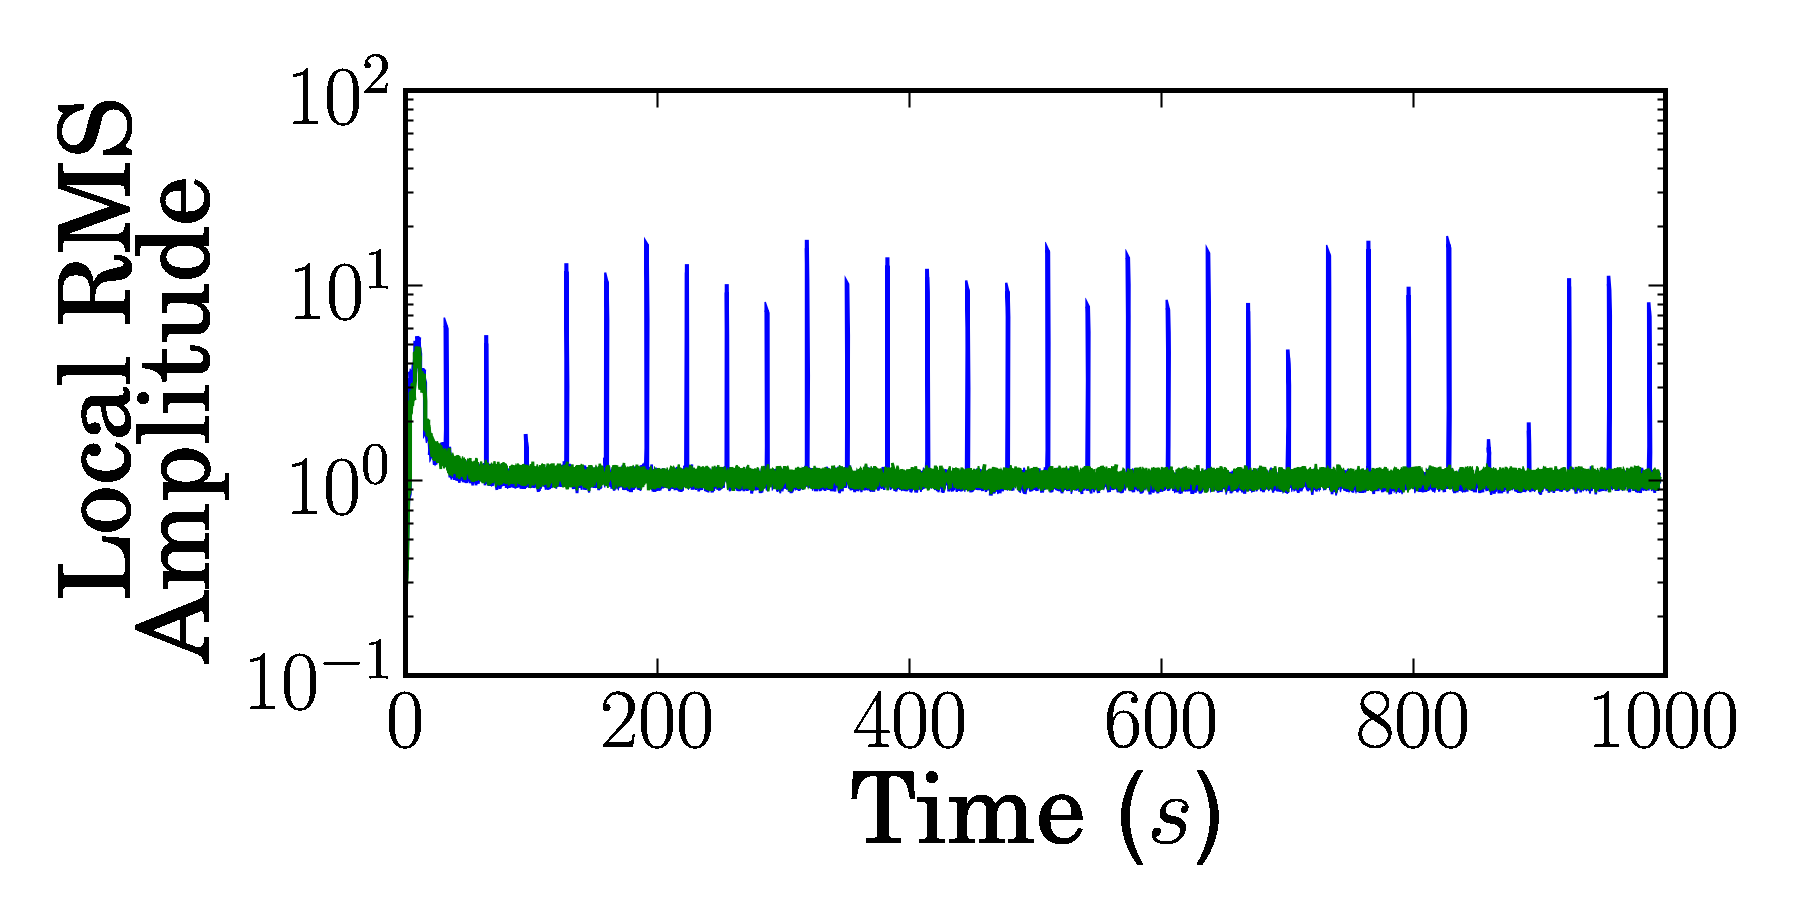
\includegraphics{figures/whiten_burst_step_100_semilogy.png}}
\end{center}

An inspiral, to leading order, has gravitational-wave frequency evolution given
by
\begin{equation}
f(t) = \frac{1}{8 \pi \mathcal{M}} \left( \frac{t_c - t}{5 \mathcal{M}} \right)^{-3/8}\;,
\end{equation}
whose time derivative is given by
\begin{equation}
\frac{df}{dt} = \frac{3}{320 \pi \mathcal{M}^2} \left( \frac{t_c - t}{5 \mathcal{M}} \right)^{-11/8}\;.
\end{equation}
Combining these, we find the frequency evolution as a function of frequency to
be
\begin{equation}
\frac{df}{dt}(f_0) = \frac{3}{320 \pi \mathcal{M}^2} \left( 8 \pi \mathcal{M} f_0 \right)^{3/11}\;,
\end{equation}
which can be inverted to get the minimum frequency which has a given frequency
derivative,
\begin{equation}
f_0 = \frac{1}{8 \pi \mathcal{M}} \left( \frac{320 \pi \mathcal{M}^2}{3} \frac{df}{dt} \right)^{11/3}\;.
\end{equation}

If we allow frequency bins to be affected by an injection only once within the
median history, we need to calculate the corresponding $df/dt$ for our PSD
calculation. An FFT of a buffer with length $T$ will have a frequency
resolution $df = 1/(2T)$. Hann windowing the data and overlapping buffers by
50\% introduces correlations in neighboring frequency bins of the FFT. This
means that we actually want the frequency to change by $df = 3/(2T)$ before the
next PSD calculation, which happens a $dt = T/2$ later, resulting in a minimum
$df/dt = 3/T^2$.

Combining these results we find the lower frequency bound for our injections,
assuming a chirp mass for a binary with $m_1 = m_2 = 1 M_{\odot}$ and $T = 8$
s, is 23 Hz.

We want to compute the equivalent injection density which would be biased as
much as lalapps\_inspiral's PSD estimator, which allows $\sim3$ injections per
2048 seconds. It computes the PSD by breaking the segment up into 16 256 second
chunks. These chunks are then combined into to sets of 8 chunks each. The
median of each set is then averaged across the sets for each frequency bin to
produce the PSD estimate for that 2048 second segment. This procedure results
in an average injection density of 1.5 per 8 PSDs in the median history, which
is comparable to LLOID's 1 per 7 PSDs in the median history. Since LLOID has an
injection history of 7 PSDs which span 32 seconds, this means LLOID can perform
one injection every 32 seconds, or 64 injections per 2048 second segment, more
than an order of magnitude increase in density over lalapps\_inspiral.
\end{comment}
